

\section{Geographical Earth Model}

\subsection{Earth Model}

The shape of the Earth has always intrigued us, leading to the development of various models over the centuries to precisely define its measurements and structure.
The primary motivation behind determining the planet's shape stems from the practical considerations of navigation, where knowledge of true distances and directions is essential.
In modern times, we not only travel from one point to another on the planet but also generate data with precise positions for further analysis of different phenomena.


Mostly, a spherical Earth comes to the mind, which is not the true shape of the Earth as shown below.

\begin{figure}[h]
    \centering
    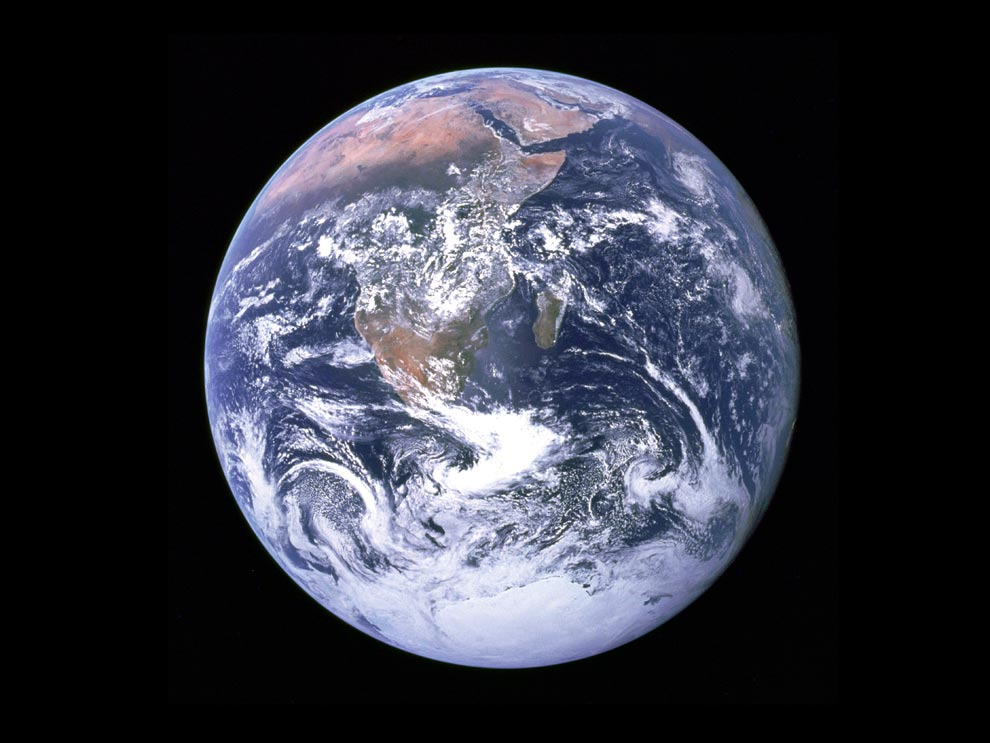
\includegraphics[width=0.5\linewidth]{figures/chapter-2/earth.jpg}
    \caption{The Blue Marble (Source \cite{EARTH_IMAGE}) }
    \label{fig:earth}
\end{figure}


To define the shape of any given surface, observations and a mathematical model are employed to establish its dimensions.
This is also true when it comes to defining the figure of the Earth, which exhibits irregularities due to variations on its surface.
Irrespective of our position on the surface of the planet, there are likely to be heights and depressions. When considering only the land mass, we can observe diverse mountain
ranges spanning the globe, defined by peaks and valleys.
With all of these irregularities, determining the true shape of the Earth becomes a difficult task.
While we may consider the oceans as a flat surface (acknowledging the presence of uneven shapes at their bottom), the issue of land mass coverage remains.

These questions surrounding the actual shape and dimensions of the Earth fall within the realm of Geodesy, a scientific field concerned with accurately measuring and
determining the Earth's geometry, orientation in space, and gravitational field.
For measuring the Earth, simpler mathematical models are defined by the geodesists which are used to capture the most obvious features of the Earth\cite{GEODESY}.

The irregular nature of our planet makes it difficult to define through mathematical models.
Consequently, there is a necessity to investigate a less complex model that portrays the Earth's rugged and uneven surface, which can be characterized by a mathematical
model and simplifies computations.

\subsection{Geoid Model}
The Earth geoid is a model that is defined by the average global sea level and is utilized for precise measurements of surface elevations \cite{NOAA_GEOID}.

This model serves as a theoretical representation that aims to address the irregularities found on the actual Earth's surface. To calculate the mean sea level (MSL),
we need to average the actual sea levels on the global level.
As the majority of the Earth is covered by oceans, but also features substantial land masses, it is crucial to account for both when conducting these calculations.
This can be achieved by hypothetically filling the land masses with oceanic waters, thereby considering the resulting water surface as the mean sea level on land. Despite the seemingly straightforward nature of constructing the geoid model, researchers are actively gathering data and developing methods to accurately depict this model.
NASA's GRACE Mission and the European Space Agency (ESA)'s GOCE missions are separately measuring the Earth's gravity field that helps in the calculations for generating the geoid model.
In the field of geodesy this geoid model plays an important role for making calculations and determine positions on the surface of the Earth. Moreover, the study of the geoid extends beyond geodesy and is also pertinent to climate research\cite{GISGEO_GEOID}. The geoid model is considered the true representation of the Earth's surface and shape.

\begin{figure}[h]
    \centering
    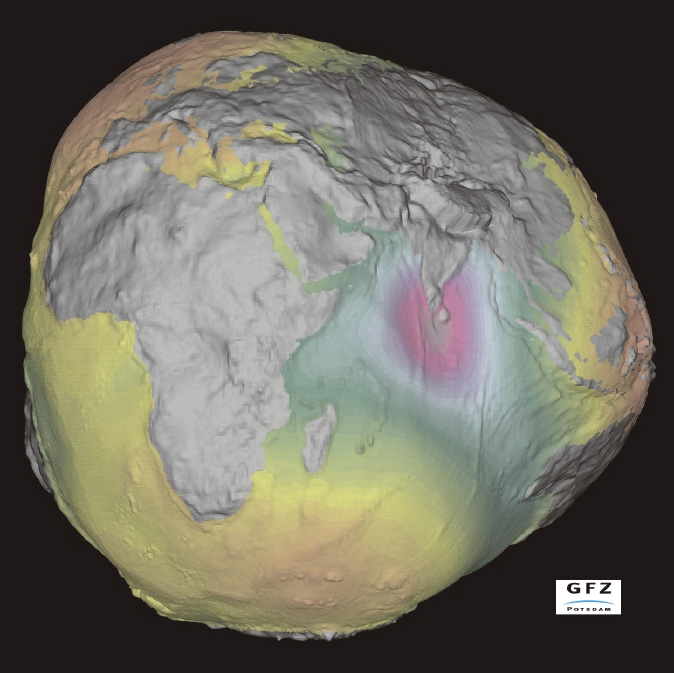
\includegraphics[width=0.7\linewidth]{figures/chapter-2/geoid.jpg}
    \caption{Geoid: The Potsdam Gravity Potato (Source \cite{GEOID_IMAGE}) }
    \label{fig:geoid-image}
\end{figure}

Still the geoid as depicted in the above image is not a smooth surface that makes it impossible for making direct calculations. Although the irregularities in the Earth's shape have been somewhat mitigated, they still persist to some extent. Thus, the need for a simpler model to accurately represent the Earth remains for geospatial data analysis.


\subsection{Spherical Model}

The notion that the Earth possesses a spherical shape was initially posited by the ancient Greeks. Aristotle proposed the idea of a spherical Earth as
mentioned by Johns et. al. in their publication "The Figure of the Earth" in 1959 \cite{Johns1959-og}.

Although, Spherical model of Earth is not a true fact but it provides a framework for gauging dimensions and establishing geographical coordinates.
The spherical model not only simplifies the underlying geoid model as it removes the irregularities of the geoid but also it eased the way to create the coordinate reference
system which depends on latitudes and longitudes.
These latitudes and longitudes are further being utilized in pointing the position of part of the Earth.
\begin{figure}[h]
    \centering
    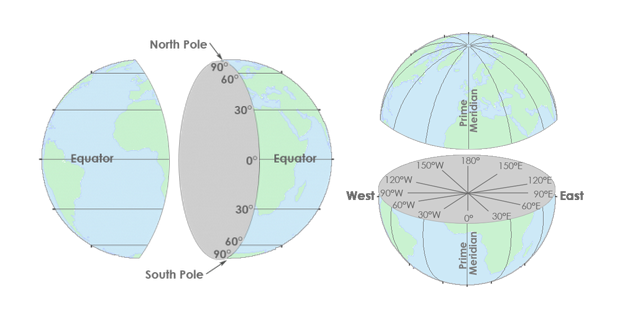
\includegraphics[width=0.7\linewidth]{figures/chapter-2/lat_lon.png}
    \caption{Depiction of Latitudes and Longitudes (Source \cite{GISGEO_LatLon}) }
    \label{fig:shpere-image}
\end{figure}

The latitudes and longitudes are calculated as angles from the equatorial line and the prime meridian respectively. By the advancement of our understanding of the shape of the earth, we have came to a conclusion that sphere is not the actual representation of the Earth. By studying the gravitational field of the Earth a
correction is needed which bring us to the representation which is now being used for not only making correct positioning of points on Earth, but this representation is also being used for creating maps.

\subsection{Ellipsoid Model}

\begin{figure}[h]
    \centering
    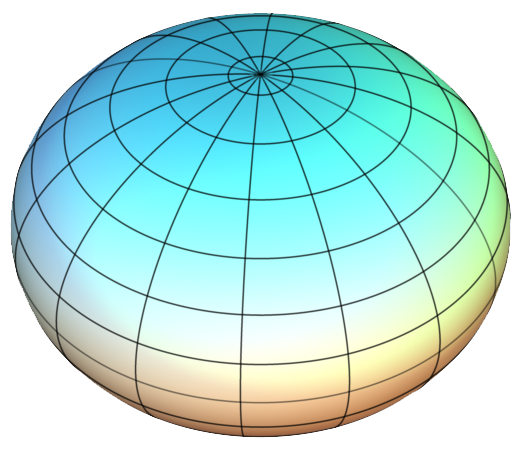
\includegraphics[width=0.4\linewidth]{figures/chapter-2/elipsoid.png}
    \caption{An Ellipsoid (Source \cite{GISGEO_Ellipsoid}) }
    \label{fig:ellipsoid-image}
\end{figure}
After the discovery of the gravitational force, Newton proposed that the Earth is a oblate spheroid or an ellipsoid. This representation of the Earth was confirmed using careful measurements \cite{Osserman2006-ys}. The Earth's ellipsoid depiction serves as a straightforward model that, much like the spherical approximation, streamlines the computations involved in analyzing geospatial data.
This model overcomes the issue of the irregular surface shape of the geoid.

\subsection{Relationship between the ellipsoid and the geoid model}
The geodesists opt for the ellipsoid model over the spherical model when establishing a coordinate reference system because it better represents the Earth's shape.

\begin{figure}[h]
    \centering
    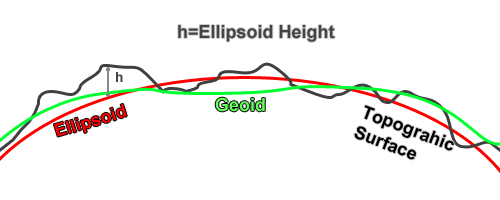
\includegraphics[width=0.6\linewidth]{figures/chapter-2/Ellipsoid-height-relation.png}
    \caption{Relationship between the geoid model and reference ellipsoid(Source \cite{GISGEO_Ellipsoid}) }
    \label{fig:relationship-ellipsoid-geoid-image}
\end{figure}

The generation of coordinate pairs is influenced by the relationship between the ellipsoid and the geoid model. A suitable reference ellipsoid is selected as a close approximation of the underlying geoid model.
When dealing with specific regions different countries use reference ellipsoids which best fit the region of the countries.
World Geodetic System (WGS84) provides a reference ellipsoid which accommodate the whole Earth's geoid \cite{GISGEO_Ellipsoid}. This reference ellipsoid brings the coordinate system (pairs of latitudes and longitudes) which is used for navigation, reference points on the Earth's surface and geospatial data is mostly collected using the coordinate system which uses the its reference ellipsoid.
GPS global positioning system uses WGS84 as well\cite{GISGEO_WGS84}.

Even though the above models approximate the shape and the dimension of the Earth, we still need the depiction of the Earth which could be used in the analysis of the geospatial data using convolutional neural networks.